% !TeX program = xelatex
% !TeX encoding = UTF-8
\documentclass[12pt, a4paper]{ctexart}

%----------------------------------------------------------------------------------------
%	1. 字体与版面设置
%----------------------------------------------------------------------------------------
\usepackage{fontspec}
\setmainfont{Times New Roman}
\setCJKmainfont[AutoFakeBold=true]{SimSun}
\usepackage{geometry}
\geometry{left=1.8cm, right=1.8cm, top=2.5cm, bottom=2.5cm, footskip=2cm}
\usepackage[table]{xcolor}

%----------------------------------------------------------------------------------------
%	封面背景所需宏包（水印已移除）
%----------------------------------------------------------------------------------------
\usepackage{tikz}
\usepackage{eso-pic}

\usepackage{setspace}
\setstretch{1.5}
\usepackage{enumitem}

%----------------------------------------------------------------------------------------
%	2. 章节格式定制
%----------------------------------------------------------------------------------------
\ctexset{
    section = {
        name = {第,章},
        number = \chinese{section},
        format = \centering\heiti\zihao{3}\bfseries,
        aftername = \quad,
        beforeskip = 1ex,
        afterskip = 1ex,
        break = \clearpage
    },
    subsection = {
        number = \thesubsection,
        format = \heiti\zihao{-3},
        beforeskip = 0.5ex,
        afterskip = 0.5ex
    },
    subsubsection = {
        number = \thesubsubsection,
        format = \heiti\zihao{4},
        beforeskip = 0ex,
        afterskip = 0ex
    },
    contentsname = {\heiti 目录}
}

%----------------------------------------------------------------------------------------
%	3. 工具宏包
%----------------------------------------------------------------------------------------
\usepackage{amsmath, amsfonts, amssymb}
\usepackage{multirow}
\usepackage{booktabs}
\usepackage{array}
\usepackage[most]{tcolorbox}
\usepackage{graphicx}
\usepackage{float}

% 【要点】高亮框（青色系）
\newtcolorbox{keybox}[1][]{
    enhanced,
    colframe=cyan!70!black,
    colback=cyan!4!white,
    fonttitle=\bfseries\sffamily,
    coltitle=black,
    title={#1},
    drop shadow,
    sharp corners=downhill,
    breakable
}
% 【发现】高亮框（红色系）
\newtcolorbox{findbox}[1][]{
    enhanced,
    colframe=red!65!black,
    colback=red!4!white,
    fonttitle=\bfseries\sffamily,
    coltitle=black,
    title={#1},
    drop shadow,
    sharp corners=downhill,
    breakable
}

%----------------------------------------------------------------------------------------
%	4. 页眉页脚
%----------------------------------------------------------------------------------------
\usepackage{fancyhdr}
\pagestyle{fancy}
\fancyhf{}
\setlength{\headheight}{15pt}
\lhead{\songti 唐宋诗词的时代回响 · 中期报告}
\rhead{\leftmark}
\renewcommand{\headrulewidth}{0.4pt}
\cfoot{\thepage}
\renewcommand{\footrule}{
    \vskip -8pt
    \begingroup
        \footnotesize\songti
        VisProject第2小组中期报告 \hfill 唐宋之变
    \endgroup
    \par
    \vskip 3pt
    \hrule width\headwidth height 0.4pt
    \vskip 3pt
}

%----------------------------------------------------------------------------------------
%	超链接
%----------------------------------------------------------------------------------------
\usepackage[
    colorlinks=true,
    linkcolor=cyan!70!black,
    urlcolor=cyan!70!black,
    citecolor=cyan!70!black,
    bookmarksnumbered=true,
    pdfstartview=FitH,
    pdftitle={唐宋诗词的时代回响 · 中期报告},
    pdfauthor={VisProject第2小组}
]{hyperref}

%======================================================================
%   文档正文开始
%======================================================================
\begin{document}

% --- 封面 ---
\begin{titlepage}
    \AddToShipoutPictureBG*{
        \begin{tikzpicture}[remember picture, overlay]
            \node[opacity=1, inner sep=0pt] at (current page.center) {
                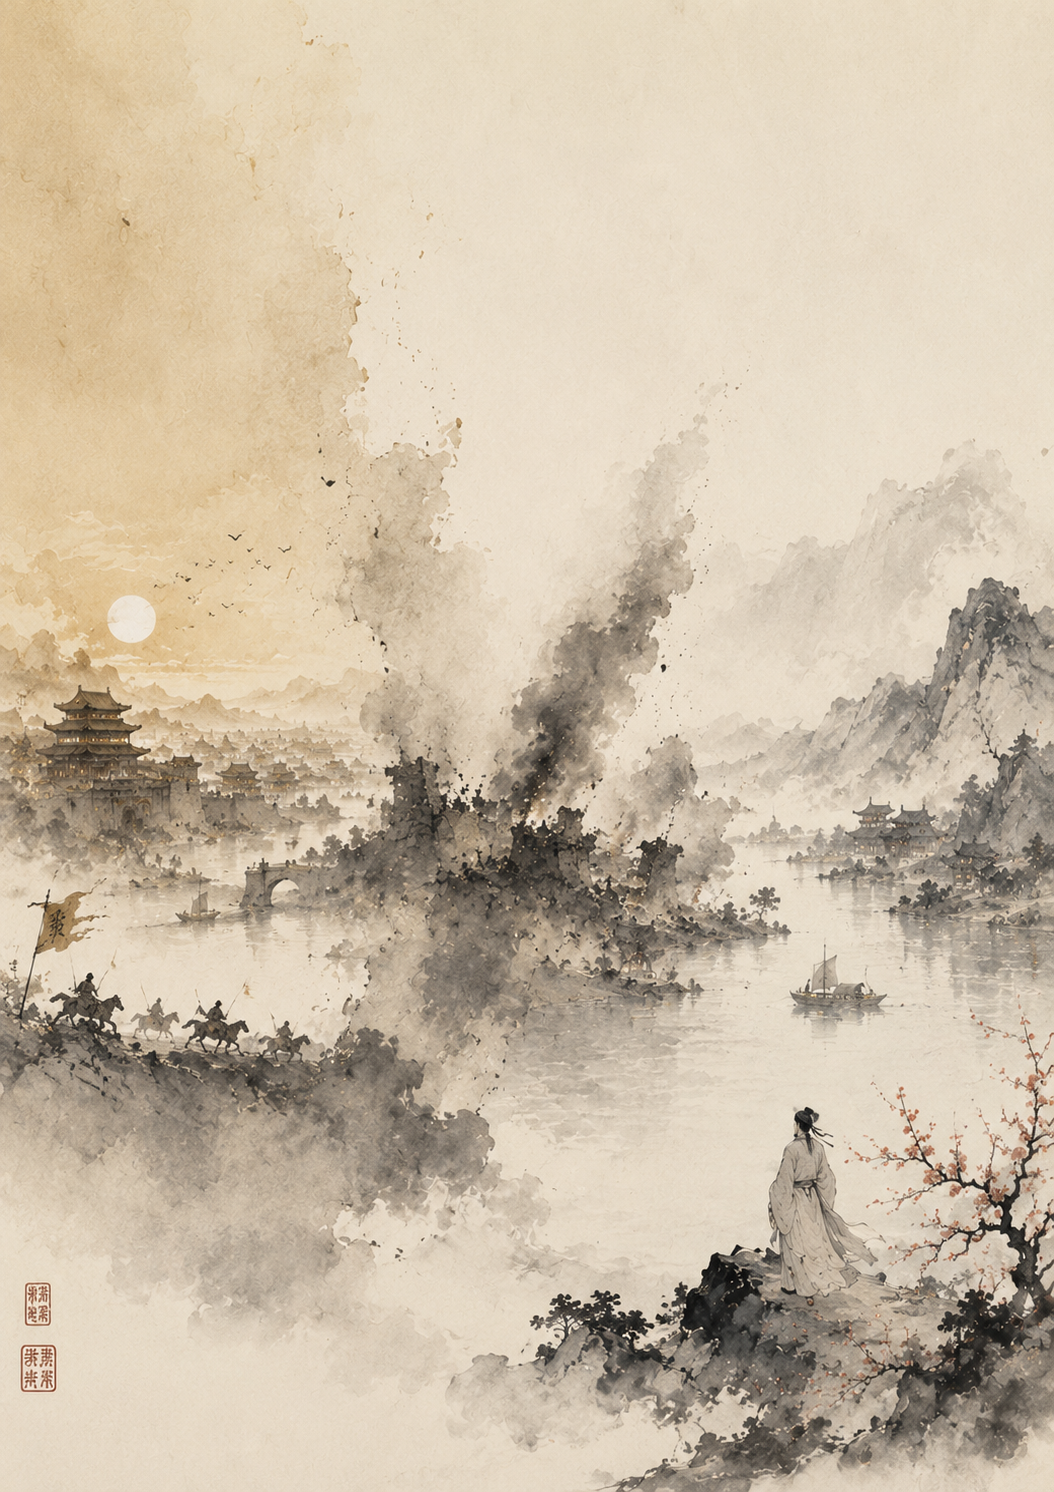
\includegraphics[width=\paperwidth, height=\paperheight]{figures/cover3.png}
            };
        \end{tikzpicture}
    }

    \begin{center}
        \vspace*{1.6cm}
        \resizebox{0.92\textwidth}{!}{
        \Huge \heiti \color{black} 唐宋诗词的时代回响} \\[0.9cm]
        \resizebox{0.88\textwidth}{!}{
        \huge \color{black} The Echoes of an Age: Tang--Song Poetry across Two Ruptures
        } \\[1.2cm]
        {\LARGE \heiti \color{black}
        以两次大断裂为锚的文本计量可视化} \\[0.6cm]
        {\large \color{black} 数据可视化导论 \quad 课程项目 VisProject \quad 中期报告}
        \vfill
        {\large \heiti \color{black} 组员：\underline{陈维嘉}\ \ \underline{蒋文倩}\ \ \underline{孙嘉泽} \\[0.4cm]}
        {\normalsize \color{white!85!black} 2026 年 6 月}
        \vspace*{1.2cm}
    \end{center}
\end{titlepage}

%======================================================================
%   前言页
%======================================================================
\newpage
\thispagestyle{empty}
\section*{前言}

唐诗与宋词是中国古典文学的两座高峰。本项目以约 7.8 万首唐诗、宋词为素材，借助文本计量与数据可视化，
考察文学如何回应时代——尤其是\textbf{安史之乱（755）}与\textbf{靖康之变（1127）}两次最剧烈的历史断裂前后，
文人的情感、意象、词汇与地理书写发生了怎样的变化。

我们刻意不预设"唐外向、宋内向"的单一结论，而让数据自己说话：盛唐的昂扬如何在断裂中沉潜，
北宋如何转向清雅内省，而靖康之后南宋的豪放又如何回潮。本中期报告记录截至目前的项目背景、分析任务、
数据处理、可视化设计方案，以及实现进展与下一步计划。

\vspace{1.2cm}
\begin{flushright}
    \large \textbf{数据可视化导论 · VisProject 第 2 小组} \\
    \normalsize 2026 年 6 月
\end{flushright}
\newpage

%======================================================================
%   目录页
%======================================================================
\newpage
\pagestyle{empty}
\tableofcontents
\clearpage
\pagestyle{fancy}

% --- 正文 ---
\setcounter{page}{1}
\pagenumbering{arabic}
\setcounter{section}{0}

\section{项目背景}

\subsection{主题}

本项目以中国古典诗词为素材，覆盖\textbf{公元 712 年（盛唐）至 1279 年（南宋末）}，跨越唐、五代、两宋，
构建一个叙事型数据可视化系统，用可量化的文本证据考察文学如何回应时代变迁。

\subsection{研究立意：探索性，而非预设结论}

我们\textbf{不预设}“唐外向、宋内向”的单一结论，而是以两次最剧烈的历史断裂为锚，做探索性分析：

\begin{keybox}[统领问题]
中国文人在两次大断裂——\textbf{安史之乱（755）}、\textbf{靖康之变（1127）}——前后，
精神世界与文学表达发生了怎样的变化？
\end{keybox}

数据已显示这并非单调的“由外向内”：唐代外向性确在下降，\textbf{但靖康之变后，南宋豪放派
（辛弃疾、陆游的家国激愤）使外向性回潮}，与姜夔、吴文英的醇雅并存——一个断裂岔出两条路。
这种“反弹”正是结论的一部分，而非噪音。

\subsection{为什么是 712–1279 这个跨度}

\begin{itemize}[leftmargin=*, itemsep=0.3em]
    \item \textbf{覆盖完整周期}：兴起—极盛—断裂—沉潜—重构—再断裂—再分化，两次“盛极而崩”互为镜像。
    \item \textbf{两大断裂可对照}：755 与 1127 都是“军事崩溃 + 被迫南迁 + 文学剧变”，并置可见文学回应历史的共性与差异。
    \item \textbf{唐诗 vs 宋词}：完成古典诗词最经典的纵向对比。
    \item \textbf{可验证}：每个转变都有可量化的文本证据（情感、意象、地理、词频多维同步）。
\end{itemize}

\subsection{历史分期：五期 + 两道断裂带}

时间轴为有序时期轴，两道断裂带分别落在 755（盛唐\,$\vert$\,中唐）与 1127（北宋\,$\vert$\,南宋）。

\begin{table}[H]
\centering
\renewcommand{\arraystretch}{1.3}
\begin{tabular}{>{\bfseries}l l l l}
\toprule
时期 & 大致时间 & 社会状态 & 文学精神 \\
\midrule
盛唐 & 712--755 & 开元盛世 & 昂扬、开阔、功业向往 \\
中唐 & 756--835 & 安史之乱后、藩镇 & 沉郁、写实、转向内省 \\
晚唐五代 & 836--960 & 衰乱、分裂 & 感伤、绮丽、向内 \\
北宋 & 960--1127 & 统一、儒学复兴 & 理性、清雅、日常审美（内向最深） \\
南宋 & 1127--1279 & 偏安、抗金 & 豪放回潮 + 醇雅并存 \\
\bottomrule
\end{tabular}
\end{table}

\noindent\textbf{两个人形节点}：杜甫横跨安史之乱（盛唐\,$\to$\,中唐），李清照横跨靖康之变（北宋\,$\to$\,南宋）——
分别是两次断裂亲历的“最亮的星”，将在可视化中作为接缝处的关键个案。

\section{分析任务定义}

\subsection{核心研究问题}

\begin{keybox}[核心问题]
中国文人在两次大断裂——安史之乱（755）、靖康之变（1127）——前后，精神世界与文学表达发生了怎样的变化？
\end{keybox}

这是一个探索性、可被数据验证的主问题，统一收敛到“两次断裂前后的对照”这条主轴。

\subsection{为什么用可视化，而非纯统计 / 机器学习}

\begin{enumerate}[label=\textbf{\arabic*.}, leftmargin=*, itemsep=0.3em]
    \item \textbf{问题是阐释性的，而非预测性的}：要回答的不是“分类准确率多高”，而是“精神世界如何随时代迁移”，
          这类人文结论需专家在历史语境中解读，单一统计量无法概括。
    \item \textbf{核心是多维度协同的时间叙事}：情感、意象、体裁、地理、词汇需在同一时间轴上同步比对，
          可视化的多视图协调（brushing \& linking）天然适配。
    \item \textbf{目标是发现 non-trivial pattern}：探索性分析依赖交互式追问（拖时间轴、点选意象、下钻原诗），
          正是可视化的 details-on-demand 优势。
    \item \textbf{指标是代理变量，需可追溯}：情感分、外内比等都是对“精神状态”的近似度量，
          必须能随时下钻回原诗验证，避免把指标当真相。
\end{enumerate}

\subsection{六个分析子任务（X 轴 = 五个有序时期）}

\begin{table}[H]
\centering
\renewcommand{\arraystretch}{1.3}
\begin{tabular}{c l l}
\toprule
编号 & 子任务 & 看什么 / 主图 \\
\midrule
T1 & 情感演化 & 盛唐高 $\to$ 中晚唐低徊 $\to$ 北宋回升 $\to$ 南宋再降 / 情感温度计 \\
T2 & 意象演化（核心） & 外内比=宏/私：唐持续下降、\textbf{南宋回弹} / 意象河流图 \\
T3 & 体裁演化 & 唐诗体裁 $\to$ 词的兴起 / 堆叠面积图 \\
T4 & 地理空间 & 塞北西域 $\to$ 江南都市 $\to$ 偏安江南 / 诗歌地图 \\
T5 & 唐宋词汇对比 & 唐大物象 vs 宋雅物小空间（繁简已统一）/ 双色词云 \\
T6 & 两大断裂断面 & 755 / 1127 前后对照、升降词、亲历名篇 / 断面专屏 \\
\bottomrule
\end{tabular}
\end{table}

\noindent T1、T2 为主线；\textbf{T6 两大断裂为戏剧高潮}；T4 为“诗歌地理学（Poetry GIS）”亮点。
全局叠加“\textbf{流}（全集聚合，显时代面貌）/ \textbf{繁星}（三百首名篇逐首，可点击下钻）”双层。

\subsection{取舍（明确删减，避免发散）}

\begin{itemize}[leftmargin=*, itemsep=0.3em]
    \item \textbf{删除典故来源热力图}：需古汉语 NER + 古籍知识图谱，工程量巨大且准确率低。
    \item \textbf{删除 LLM 精确年份推断}：易幻觉；改用“有序时期 + 置信度”。
    \item \textbf{LLM 降为可选附件}：确定性管道为可信核心，LLM 因一致性问题默认不接入主结论。
    \item \textbf{有余力再做}：LDA 主题河流、诗人社交网络。
\end{itemize}

\section{数据说明}

\subsection{数据来源}

语料取自开源的 \textit{chinese-poetry} 数据集。

\begin{table}[H]
\centering
\renewcommand{\arraystretch}{1.3}
\begin{tabular}{l l c r}
\toprule
语料 & 文件 & 字形 & 规模 \\
\midrule
全唐诗 & \texttt{poet.tang.*.json} & 繁体 & 57\,599 首 \\
宋词（全宋，含南宋） & \texttt{ci.song.*.json} & 简体 & 21\,049 首 \\
唐作者元数据 & \texttt{authors.tang.json} & 繁体 & 3\,663 人 \\
宋词作者元数据 & \texttt{author.song.json} & 简体 & 1\,529 人 \\
名篇选集 & 唐诗三百首(366)、宋词三百首(280) & --- & --- \\
\bottomrule
\end{tabular}
\end{table}

\noindent\textbf{不使用}：\texttt{poet.song.*}（是宋诗，非宋词）、\texttt{authors.song.json}（宋诗作者）。

\subsection{两个地基性事实（决定了整套处理）}

\begin{findbox}[事实一：繁简割裂]
唐诗为\textbf{繁体}、宋词为\textbf{简体}（实测唐诗繁/简 $\approx$ 5554/30，宋词 $\approx$ 0/7304）。
若不统一，词频/意象的“唐宋对比”会把\textbf{繁简差异误当时代差异}。
\end{findbox}

\begin{findbox}[事实二：逐首创作年不可恢复]
唐 3663 位作者中能从传记解析真实生卒年者极少；逐首诗的精确创作年学界亦常存争议。
故\textbf{时间轴只能到“时期”粒度}，不伪造逐年数据。
\end{findbox}

\subsection{确定性处理管道}

管道 \texttt{ingest $\to$ metrics $\to$ qa}（详见 \texttt{pipeline/README.md}），完全确定性、可复现、不依赖大模型。

\begin{enumerate}[label=\textbf{\arabic*.}, leftmargin=*, itemsep=0.3em]
    \item \textbf{繁简归一}：作者名与正文统一经 OpenCC 繁$\to$简，统计基于简体文本，保留原文供展示。
    \item \textbf{定年阶梯}（不伪造年份）：唐——“诗人$\to$时期”查表（高置信）$\to$ 作者传记年号推时期（中置信）$\to$ 否则“未定年”；
          宋词——“宋词人$\to$北宋/南宋”查表 $\to$ 传记生年阈值 1085 $\to$ 否则“未定年”。未定年不进时间轴，但仍进唐宋对比、词频、意象聚合。
    \item \textbf{去重、空正文过滤、稳定 ID}（词无 ID 用内容哈希生成）。
    \item \textbf{名气标记}：是否入选三百首、是否名家、是否两大断裂亲历名篇。
\end{enumerate}

\subsection{时期分布（语料 78\,648 首）}

\begin{table}[H]
\centering
\renewcommand{\arraystretch}{1.25}
\begin{tabular}{l r @{\hspace{2cm}} l r}
\toprule
时期 & 数量 & 定年来源 & 数量 \\
\midrule
盛唐 & 8\,870 & 诗人表 & 33\,860 \\
中唐 & 19\,132 & 传记年号 & 9\,775 \\
晚唐五代 & 15\,633 & 宋词人表 & 8\,688 \\
北宋 & 3\,680 & 传记生年 & 3\,047 \\
南宋 & 8\,055 & 未知（未定年） & 23\,278 \\
未定年 & 23\,278 & & \\
\bottomrule
\end{tabular}
\end{table}

\noindent 可入时间轴（datable）：\textbf{55\,370 / 78\,648 $\approx$ 70\%}（唐诗 75\%；名家名篇范围接近全可定年）。

\subsection{仪表盘数据契约}

时间轴为有序时期（非年份桶）。所有文件为严格 JSON。主要产物：
\texttt{meta}、\texttt{sentiment\_by\_period}、\texttt{imagery\_flow}、\texttt{genre\_by\_period}、
\texttt{word\_freq\_comparison}、\texttt{place\_geo}、\texttt{stars}（繁星=名篇逐首）、
\texttt{rupture\_755} / \texttt{rupture\_1127}（两大断裂断面）。
分析范围可切换 \texttt{full}（流）/ \texttt{representative}（名家，叙事默认）/ \texttt{anthology}（三百首）。

\subsection{已知局限}

\begin{itemize}[leftmargin=*, itemsep=0.2em]
    \item 情感/意象为词典法\textbf{代理指标}，不如人工细读精准，但确定性、可复现，且可下钻原文核对。
    \item 未定年约 2.3 万首（多为长尾小作者）不进时间轴；时间轴结论主要由名家名篇范围支撑。
    \item 三百首选集反映后世编选取向，故保留 \texttt{full} 全集范围交叉对照。
    \item “唐诗 vs 宋词”对比同时含“诗/词体裁”与“时代”两重差异，解读时需说明。
\end{itemize}

\section{设计方案}

\subsection{设计需求}

围绕核心问题，系统需满足：

\begin{enumerate}[label=\textbf{\arabic*.}, leftmargin=*, itemsep=0.25em]
    \item \textbf{叙事性}：以时间长河为骨架，把情感、意象、体裁、地理、词汇组织成一条可被引导阅读的故事线。
    \item \textbf{多视图协调}：各视图共享同一时期语义，支持 brushing \& linking——选定一个时期，其余视图同步聚焦。
    \item \textbf{细节按需展开}：宏观指标可下钻到具体诗作，保证代理指标可追溯回原文。
    \item \textbf{对比性}：支持“唐 vs 宋词”纵向并置，以及两大断裂前后的断面对照。
    \item \textbf{数据诚实}：低置信 / 未定年数据在视觉上弱化或单列，不冒充事实。
\end{enumerate}

\subsection{视觉隐喻：时间长河上的“流”与“繁星”}

\begin{table}[H]
\centering
\renewcommand{\arraystretch}{1.3}
\begin{tabular}{l l l}
\toprule
隐喻 & 数据层 & 视觉角色 \\
\midrule
流（普通作品汇聚成时代面貌） & 全集按时期聚合 & 连续成势的底层河水 \\
繁星（最具代表性的名篇） & 三百首名篇逐首 & 河面上可点击下钻的星 \\
\bottomrule
\end{tabular}
\end{table}

\noindent 两道红色“断裂带”（755、1127）横切长河，标记安史之乱与靖康之变。

\subsection{技术栈}

\textbf{React + Vite + ECharts}（前端，纯静态数据，无后端）。理由：规划的图表（themeRiver、地图、词云、堆叠面积、关系图）
几乎都是 ECharts 原生类型，开箱即用；数据已是静态 JSON，\texttt{fetch} 即用、可构建为静态包演示；组件化便于三人并行开发。

\subsection{六屏叙事结构}

\begin{table}[H]
\centering
\renewcommand{\arraystretch}{1.25}
\begin{tabular}{c l l l}
\toprule
屏 & 主题 & 主图 & 交互 \\
\midrule
S1 & 历史时间轴 + 情感温度计 & 折线 + 事件带 & 拖时间轴联动 \\
S2 & 意象的生死流转（核心） & 意象河流图 + 外内比 & 点选意象高亮 \\
S3 & 诗体的新陈代谢 & 堆叠面积 & hover 看明细 \\
S4 & 地域空间（Poetry GIS） & 地图 + 散点/热力 & 切时期看版图 \\
S5 & 唐诗 vs 宋词 & 双色对比词云 & 点词下钻例句 \\
S6 & 两大断裂断面 & 前后对照 + 升降词 & 切换 755 / 1127 \\
\bottomrule
\end{tabular}
\end{table}

\subsection{多视图协调}

S1 的时间轴是全局“指挥棒”：选定时期后，S2 河流聚焦该时段、S3 体裁高亮对应列、S4 地图切到该时期版图，
实现视图间真正联动而非各自独立——这是评分中“多视图协调与交互”的核心着力点。

\section{实现进展与待完成工作}

\subsection{目前实现进展}

\subsubsection{数据处理管道（已完成并通过校验）}

已完成从原始数据集到仪表盘数据的\textbf{完整确定性管道}（\texttt{config / normalize / ingest / metrics / qa}），
并对旧版做了地基级重构：

\begin{enumerate}[label=\textbf{\arabic*.}, leftmargin=*, itemsep=0.3em]
    \item \textbf{繁简统一}：OpenCC 繁$\to$简，唐宋词频对比首次干净（不再把繁简差异误当时代差异）。
    \item \textbf{诚实定年}：弃用旧“作者生卒中点分 20 年桶”（被默认年份污染），改为有序时期轴 + 定年阶梯，唐诗可定年 $\approx$ 75\%。
    \item \textbf{范围纠错}：发现宋词语料实为全宋词（含大量南宋），改用词人表 + 生年阈值区分北宋/南宋。
\end{enumerate}

\begin{keybox}[端到端校验（qa.py 全部通过）]
语料 78\,648 首；datable 70\%；\textbf{简体文本繁体残留 = 0}；所有仪表盘 JSON 严格可解析；
时期序列按 盛唐$\to$中唐$\to$晚唐五代$\to$北宋$\to$南宋 单调；去重与定年对账一致。
\end{keybox}

\subsubsection{初步分析发现（核心结果）}

确定性指标已能复现并量化核心叙事，且在 \texttt{full} 与 \texttt{representative} 两个范围下趋势一致（结论稳健）。

\begin{figure}[H]
    \centering
    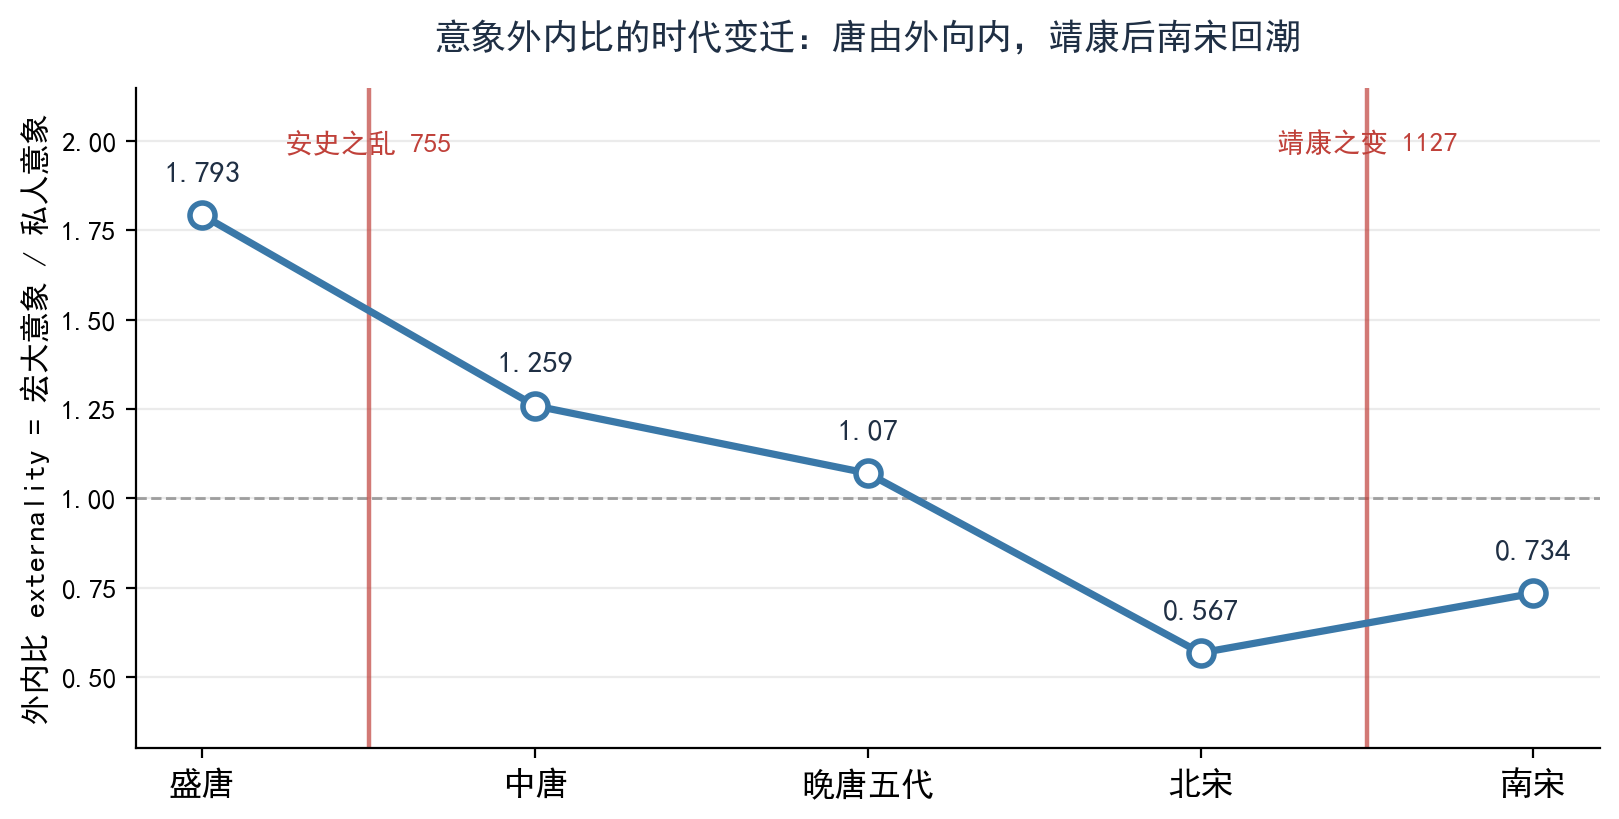
\includegraphics[width=0.92\textwidth]{figures/fig_externality}\\[4pt]
    {\small\heiti 图 1\quad 意象外内比（宏大意象 / 私人意象）的时代变迁}
\end{figure}

\begin{findbox}[关键发现]
外内比：盛唐 1.79 $\to$ 中唐 1.26 $\to$ 晚唐 1.07 $\to$ 北宋 0.57 $\to$ \textbf{南宋 0.73（回升）}。
唐代“由外向内”清晰可见，北宋内向最深；而\textbf{靖康之变后南宋外向性回潮}——
辛弃疾、陆游的家国激愤使“万里/西风”等宏大意象反弹。这一“反弹”是单调“外$\to$内”叙事无法解释的，
正是本项目最有价值的发现。
\end{findbox}

\begin{figure}[H]
    \centering
    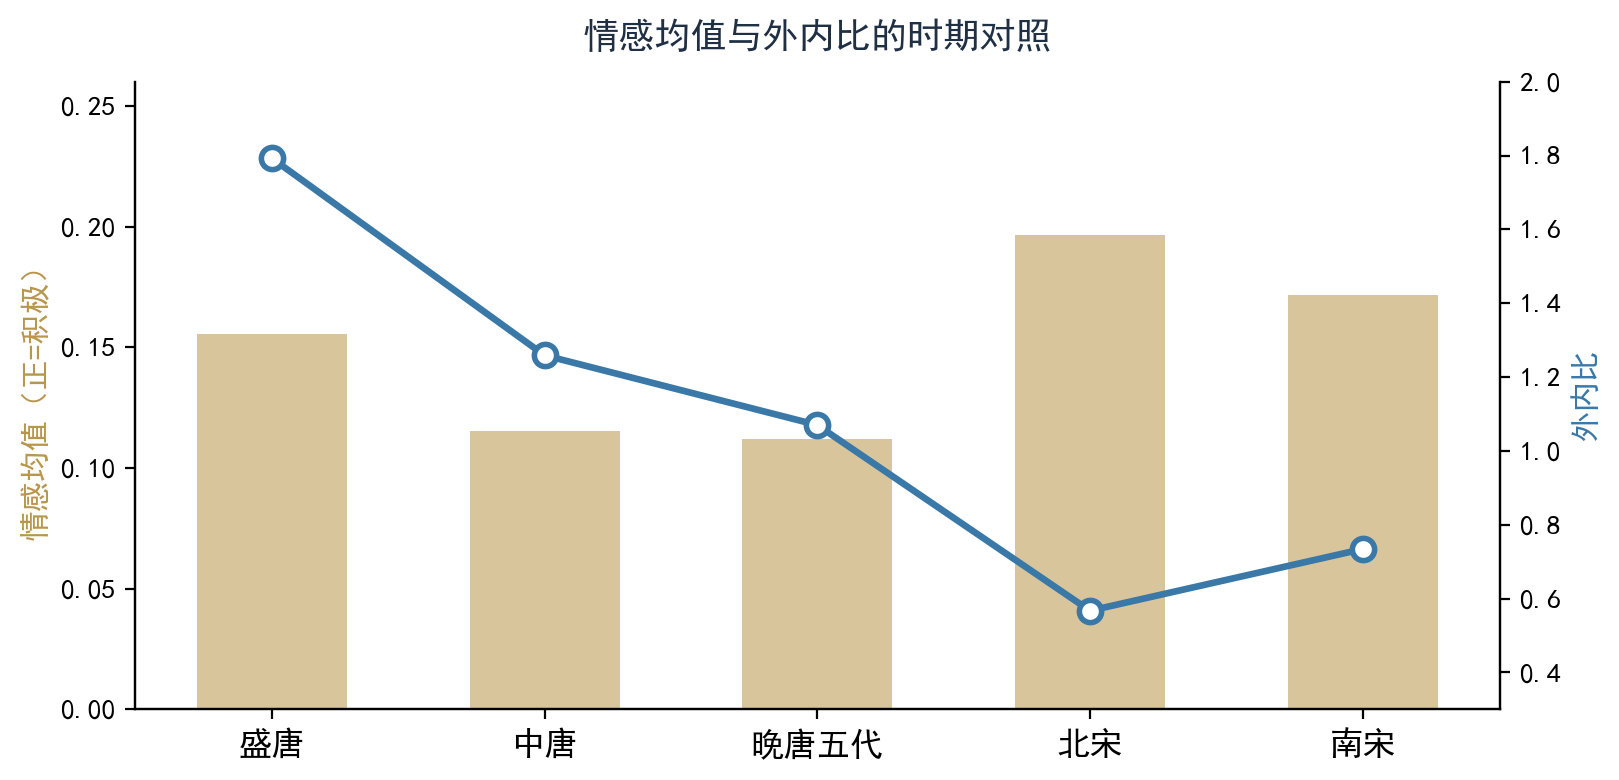
\includegraphics[width=0.92\textwidth]{figures/fig_sentiment}\\[4pt]
    {\small\heiti 图 2\quad 情感均值与外内比的时期对照}
\end{figure}

此外：两大断裂断面已自动产出——靖康断面中南宋升频词含“万里/西风/家国”信号，
策展名篇精准命中辛弃疾《永遇乐·京口北固亭》、陆游、岳飞等；唐宋独有词在繁简统一后呈清晰分野
（唐“心/身/城/门/名”偏外、实，宋“东风/江南/梅花/归去/回首”偏婉约、私人）。

\subsubsection{文档与封面}

项目报告（背景/任务/数据/设计）、数据处理记录、\texttt{pipeline/README} 均已就绪；
本报告主题封面（水墨时间长河 + 繁星 + 两大断裂）为自制。

\subsection{待完成的工作}

\begin{enumerate}[label=\textbf{\arabic*.}, leftmargin=*, itemsep=0.3em]
    \item \textbf{前端仪表盘}：用 React + Vite + ECharts 渲染六屏叙事，落地“流 + 繁星”双层、
          两大断裂断面屏与诗歌地图，并实现多视图联动。
    \item \textbf{案例展示}：待系统跑通后补充真实截图与可复现的交互路径（如下钻杜甫安史名篇、辛弃疾靖康名篇）。
    \item \textbf{细节优化}：词频加停用词表（滤“了/是”等虚词）；宋词三百首匹配率（约 76\%）改首句匹配提升。
    \item \textbf{可选增强}：LDA 主题河流、诗人社交网络（有余力再做）；LLM 作为可选附件做细腻情感类型标注。
    \item \textbf{系统文档与答辩}：期末补齐设计需求/介绍/案例/AI 使用声明，准备 Demo 视频与现场演示。
\end{enumerate}


\end{document}
